\section*{\textbf{Question 1:}}


The table below shows the situation of 2030, considering that the coal plants are reduced to 50\% of their rated outputs.
It is clear from the table that there is enough generation in zone 1 to meet the demand of  12 TWh. But since the output of the wind farm is dependent on the wind speed, it is definitely a challenge to make sure that the energy balance at each inst ace is satisfied.\\
Whereas in zone two if the coal plant's output is reduced there seems to a shortfall of energy to meet the demand. 


\begin{table}[H]
\centering
\begin{tabular}{|l|l|l|l|c|}
\hline
\multicolumn{5}{|c|}{Zone 1}                                                   \\ \hline
               & Offshore & Biomass & Coal & \multicolumn{1}{l|}{Demand (TWh)} \\ \hline
Available(TWh) & 5.6      & 1       & 7.5  & \multirow{2}{*}{12}               \\ \cline{1-4}
Used (TWh)     & 5.6      & 1       & 5.6  &                                   \\ \hline
\multicolumn{5}{|c|}{Zone 2}                                                   \\ \hline
               & Solar    & Hydro   & Coal & \multicolumn{1}{l|}{Demand (TWh)} \\ \hline
Available(TWh) & 3.6      & 0.011   & 0.32 & \multirow{2}{*}{4.8}              \\ \cline{1-4}
Used (TWh)     & 3.6      & 0.011   & 1.19 &                                   \\ \hline
\end{tabular}
\end{table}
\section*{\textbf{Question 2:}}
To overcome the problem of intermittancy in zone 1, there has to be an either a grid level storage mechanism or local storage. In case of a network congestion, there must be an infrastructure of demand side management which can clear the congestion by disconnecting/reducing the loads with lower priority.
Similar steps have to be taken in zone 2, but before implementing them there has to be an interconnection made between zone 1 and zone 2 so as to cater the demand in zone 2. This can be done through the means of looped or meshed network.
\section*{\textbf{Question 3:}}

Hours=$\frac{{{E}_{Hydro}}(GWh)}{{{P}_{Hydro}}(MW)}$
\\
Hence hydro can only be run for 18.33 hours in total.So the reservoir can be recharged once in two days, so as to cater to the diurnal variations because of solar production.





\section*{\textbf{Question 4:}}
 Based on the previous questions, it is quite evident that there is a need of storage services. Considering the issues mentioned here, storage technology has following impact:
 \begin{itemize}
     \item  Grid Congestion - In absence of storage, the existing grid connection will face problems in meeting the increasing load demands. Having storage services in the grid, reduces the stress on the grid and supplies the demand. This makes sure that the grid does not get congested. Peak shaving and peak shifting can be implemented.
     \item Reliability - Having more storage technologies essentially increases the reliability of the system. In times of less or no generation from renewable sources, storage of energy acts as a back-up and make sure the demand is met.
     \item Grid Architecture -  Introduction of storage in the grid, there will be a necessity to make the grid more "smart" i.e. using information and communication technology and better data handling. In addition to this there will be  more smaller grids for e.g. micro-grids/nano-grids. The grid architecture will not be radial anymore but more meshed/looped structure.
     \item Integration of sustainable resources - Storage will make the integration of sustainable resources more smoother. It will make sure that there is no mismatch.
     \item Ancillary Services - Introduction of ESAAS (Energy Storage as a Service). There can also be markets of reserves where storage can be used. 
 \end{itemize}     
\section*{\textbf{Question 5:}}
Based on the information for both the zones, it is possible to achieve the closure of half coal plant in zone 1 but not in zone 2. For zone 2 another possible approach is connecting zone 1 and 2 in a meshed/looped structure as mentioned in solutions to question 2. And making sure that the off-shore wind plant in zone 1 also provides energy to zone 2, thereby reducing the dependency on coal plants to zero.  
\section*{\textbf{Question 6:}}
 Without a pumped hydro power plant there will be a need of other storage methods or the demand will not be met due to the indeterminacy of the solar energy. The salt mine can be an option for compressed air storage. Taking into consideration the topography of the island it is advisable to have a pumped hydro storage in order to guard against a natural calamity (flooding).
 
\section*{\textbf{Question 7:}}
As per the Base Case, peak load and grid structure demand for Zone 1 is 250MW (connected in looped structure) whereas for Zone 2 is 98MW (connected in radial structure). 

For the year 2030, the peak loads of both the zones are expected to be 200MW and 800MW for Zone 1 and Zone 2 respectively.

This increase in supply in zone 2 (800 MW) requires Z2 to have N-1 security criterion compulsory as the supply to this area is above 100 MW. Hence,radial configuration is not preferred as it cannot satisfy N-1 redundancy. The configuration must be changed to looped or meshed network. Looped structure provides N-1 security and with the use of meshed structure, N-2 security is possible to achieve. However, meshed structure is more expensive but provides more security.\\
The grid structure in Z1 doesn't need to be changed as the peak demand has reduced from the Base Case and also looped structure provides the required N-1 security.

\section*{\textbf{Question 8:}}
The cost versus the distance (in kms) graph shown in Figure \ref{fig:AC_DC} helps in deciding on the type of connection of the overhead transmission system. Based on the data sheet for scenario 2030, the distance between island hydro plant and zone Z2 is 150km and the distance between the wind farm and Zone Z1 is 55 km and the distance between the zones Z1 and Z2 is 80 km. In all three case the distance is less than 700km - which from the Figure \ref{fig:AC_DC} indicates that an AC connection is cost effective. Considering that both zones have residential and industrial loads both the zones can be at 220kV voltage levels. This will avoid the need for stepping-down of voltage at Zone 2 (previously at 110kV). The entire network will operate at a single voltage level.
\begin{figure}[H]
    \centering
        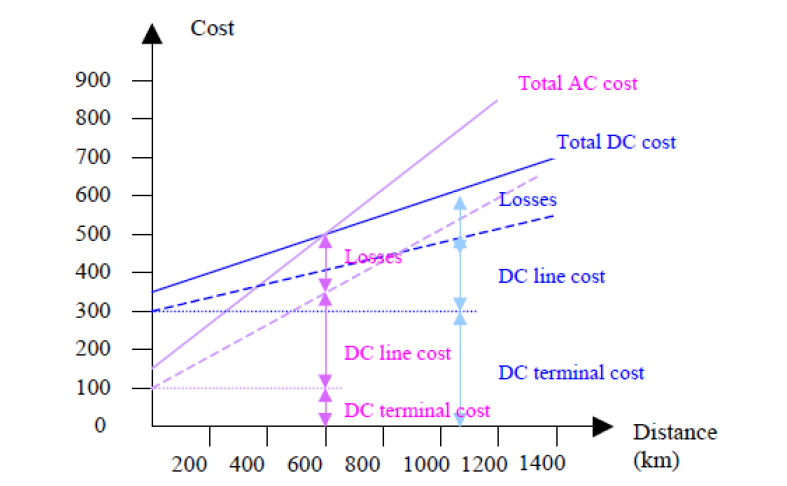
\includegraphics[width=0.8 \linewidth]{AC_DC_distance.png}
        \caption{Investment costs for an overhead line transmission system with HVAC and HVDC}
        \label{fig:AC_DC}
\end{figure}
\section*{\textbf{Question 9:}}
\begin{equation}
Power density (PD) =\frac{250(W)}{1.5({{m}^{2}})}
\end{equation}

Area required in km = $\frac{1200*{{10}^{6}}(W)}{pd}= 7320 km^2$









